\documentclass[t]{beamer}

\usetheme{Air}
\usepackage{graphics}
\usepackage{graphicx}
\graphicspath{{../images/}{../diagrams/}{.}}
%\usepackage{caption}
\usepackage{amsthm}
%\usepackage{thumbpdf}
\usepackage{wasysym}
\usepackage{ucs}
\usepackage[utf8]{inputenc}
\usepackage{pgf}
\usepackage{verbatim}
\usepackage{tikz}
\usepackage{pgfmath}
\usetikzlibrary{calc}
\usetikzlibrary{backgrounds}
\usetikzlibrary{arrows}
\usetikzlibrary{shapes.arrows}
\usetikzlibrary{shapes.geometric}
\usetikzlibrary{decorations.markings}
\usetikzlibrary{positioning}
\usetikzlibrary{fit,chains}
\usepackage{natbib}
\usepackage{wasysym}
\usepackage{soul} 
\bibliographystyle{apalike}  

%\usepackage[bottom, ragged]{footmisc}
%\usepackage{pstricks}
%\newpsobject{psid}{psline}{linestyle=dotted,dotsep=1pt}
%\newpsobject{pspsi}{psline}{doubleline=true}
%\newpsobject{pssigma}{psline}{linewidth=1.5pt}

%\usepackage{pgfpages}
%\setbeamertemplate{note page}[plain]
%\setbeameroption{show notes on second screen=right}
%http://tex.stackexchange.com/questions/21777/is-there-a-nice-solution-to-get-a-presenter-mode-for-latex-presentations

\newcommand{\beq}{\begin{equation}}
\newcommand{\eeq}{\end{equation}}
\newcommand{\beqa}{\begin{eqnarray}}
\newcommand{\eeqa}{\end{eqnarray}}
\newcommand{\bi}{\begin{itemize}}
\newcommand{\ei}{\end{itemize}}
\newcommand{\ket} [1] {\vert #1 \rangle}
\newcommand{\bra} [1] {\langle #1 \vert}
\newcommand{\braket}[2]{\langle #1 | #2 \rangle}
\newcommand{\ev}[1]{\langle #1 \rangle}
\newcommand{\vbra}[1]{\left ( #1 \right |}
\newcommand{\vket}[1]{\left |#1 \right )}
\newcommand{\vbraket}[2]{\left ( #1 \middle |#2 \right )} 
\newcommand{\braopket}[3]{\left \langle #1 \middle |#2 \middle | #3 \right \rangle} 
\newcommand{\vbraopket}[3]{\left ( #1 \middle |#2 \middle | #3 \right )} 

%\newcommand<>{\highlighton}[1]{%
%  \alt#2{\structure{#1}}{{#1}}
%}

\newcommand{\icon}[1]{\pgfimage[height=1em]{#1}}

\usepackage{empheq}

\newlength\mytemplen
\newsavebox\mytempbox

\makeatletter
\newcommand\mybluebox{%
    \@ifnextchar[%]
       {\@mybluebox}%
       {\@mybluebox[0pt]}}

\def\@mybluebox[#1]{%
    \@ifnextchar[%]
       {\@@mybluebox[#1]}%
       {\@@mybluebox[#1][0pt]}}

\def\@@mybluebox[#1][#2]#3{
    \sbox\mytempbox{#3}%
    \mytemplen\ht\mytempbox
    \advance\mytemplen #1\relax
    \ht\mytempbox\mytemplen
    \mytemplen\dp\mytempbox
    \advance\mytemplen #2\relax
    \dp\mytempbox\mytemplen
    \fcolorbox{airlightblue}{white}{\hspace{1em}\usebox{\mytempbox}\hspace{1em}}}

\makeatother

\tikzset{peps/.style={circle=2pt,draw=black!100,fill=green!50,inner sep=3pt}}
\tikzset{bpeps/.style={circle=2pt,draw=black!100,thick,fill=green!50,inner sep=3pt}}
\tikzset{gamma/.style={circle=2pt,draw=black!100,fill=blue!20,inner sep=3pt}}
\tikzset{lambda/.style={rectangle,rotate=45,draw=black!100,fill=orange!50,inner sep=4pt}}
\tikzset{operator/.style={circle=2pt,draw=black!100,fill=orange!80,inner sep=3pt}}
\tikzset{cdot/.style={circle=2pt,draw=black!100,fill=white,inner sep=1pt}}
\tikzset{bg/.style={rounded corners,thin,fill=blue!10}}
\tikzset{inv/.style={opacity=0}}
\tikzset{spin/.style={circle=2pt,draw=black!100,fill=orange!80,inner sep=3pt}}
\tikzset{unitbox/.style={fill=black!3,rounded corners}}
\tikzset{corner/.style={rectangle=10pt,fill=blue!50,draw=black}}
\tikzset{side/.style={rectangle=6pt,fill=blue!20,draw=black}}
\tikzset{cside/.style={circle=6pt,fill=blue!20,draw=black}}
\tikzset{swapg/.style={circle=1pt,draw=black,fill=black!80,inner sep=1pt}}

\tikzset{base/.style={circle=2pt,fill=orange!80,draw=black}}
\tikzset{det/.style={circle=2pt,fill=blue!20,draw=black,inner sep=4pt}}
\tikzset{iso/.style={circle=2pt,fill=red!20,draw=black,inner sep=4pt}}
\tikzset{top/.style={circle=2pt,fill=black!20,draw=black,inner sep=4pt}}
\tikzset{siso/.style={circle=1pt,fill=red!20,draw=black,inner sep=1pt}}

%Brayden's
\tikzset{GHZ/.style={circle=2pt,fill=black!80,draw=black,inner sep=2pt}}
\tikzset{X/.style={circle=2pt,fill=black!80,text=white,font=\footnotesize, draw=black,inner sep=1pt}}
\tikzset{W/.style={circle=2pt,fill=black!20,draw=black,double,inner sep=2pt}}
\tikzset{eli/.style={ellipse, rotate=0, draw=black, fill=gray!20}}

%http://tex.stackexchange.com/questions/199683/how-to-plot-quantum-logical-gates-with-tikz
\tikzset{
cross/.style={path picture={ 
            \draw[thick,black](path picture bounding box.north) -- (path picture bounding                  box.south) (path picture bounding box.west) -- (path picture bounding                      box.east);
            }},
crossx/.style={path picture={ 
            \draw[thick,black,inner sep=0pt]
                (path picture bounding box.south east) -- (path picture bounding box.north west) (path picture bounding box.south west) -- (path picture bounding box.north east);
            }},
circlewc/.style={circle=2pt,draw, crossx}
}
%\newtheorem{LSM}{{\em Theorem: Lieb, Schultz, Mattis (1961)}}
%\newtheorem{Oshikawa}{{\em Extension: Oshikawa (1999)}}

\pdfinfo
{
  /Title       (Entanglement in Featureless Mott Insulators)
  /Creator     (TeX)
  /Author      (Brayden Ware)
}


\title{Entanglement in Featureless Mott Insulators}
%\subtitle{}
\author{Brayden Ware}
\date{March 6th 2014}

%\includeonly{slides/LSM1}
\begin{document}

\frame{\titlepage}


%%%%%%%%%%%%%%%%%%%%%%%%%%%%%%%%%%%%%%%%%
%%%%%%%%%% Pre-outline section %%%%%%%%%%
%%%%%%%%%%%%%%%%%%%%%%%%%%%%%%%%%%%%%%%%%
% \section*{}

% \begin{frame}{Frame Title}
\vskip-1.5cm

\end{frame}

%%%%%%%%%%%%%%%%%%%%%%%%%%%%%%%%%%%%%%%%%
%%%%%%%%%% Outline code %%%%%%%%%%%%%%%%%
%%%%%%%%%%%%%%%%%%%%%%%%%%%%%%%%%%%%%%%%%
\section*{}

\begin{frame}
  \frametitle{Outline}
  \vskip-1.5cm
  \tableofcontents
\end{frame}

\AtBeginSection[]
{
\frame{
  \vspace{2cm}
  {\huge \insertsection}
  }
}
%\AtBeginSection[]
%{
%  \frame<handout:0>
%  {
%    \frametitle{Outline}
%    \vskip-1.5cm
%    \tableofcontents[currentsection]
%  }
%}

%\AtBeginSubsection[]
%{
%  \frame<handout:0>
%  {
%    \frametitle{Outline}
%    \tableofcontents[sectionstyle=show/hide,subsectionstyle=show/shaded/hide]
%  }
%}
%%%%%%%%%%%%%%%%%%%%%%%%%%%%%%%%%%%%%%%%%
%%%%%%%%%% Content starts here %%%%%%%%%%
%%%%%%%%%%%%%%%%%%%%%%%%%%%%%%%%%%%%%%%%%

\section{Motivation}
\begin{frame}{Featureless Insulators}
\vskip-1.5cm

\tikzstyle{na} = [baseline=-1ex]
\tikzstyle{every picture}+=[remember picture]
\def\tikzoverlay{
   \tikz[overlay, na] \node
}

\begin{columns}[T]
    \begin{column}[T]{.6\textwidth}
           \begin{block}<1->{Definition of `Featureless Insulator'}
            %\vskip-1em
            \bi
                % 0 T G.S. of quantum Hamiltonians
            \item Gapped \tikzoverlay  (tail1) {}; 
              
                %Energy gap to excitations
                %Has no gapless modes
            \item Symmetric \tikzoverlay  (tail2) {}; 
                %G.S. Wavefunction preserves all symmetries of the
                % Hamiltonian, no local order parameter
								% Has no spontaneous symmetry breaking
								% Context is lattice Hamiltonians with U(1) symmetry which 	
								% I'll refer to as charge conservation symmetry (could be spin)
								% Discrete translation as well as lattice rotations
            \item No topological order \tikzoverlay  (tail3) {}; 
                %exotic statistics
            \ei
            \end{block}
            \begin{block}<1->{Alternate Definition}
            \vskip-1em 
           	 \bi
           	 \item Unique %fixed gap% 
           	 ground state on \hskip4em all
        		 boundary-less systems
        		 \item Possibly with 'features' \hskip4em localized 
        					to edge of system
        					%Features means gapless edge modes, spontaneous symmmetry
        					%breaking, or edge topological order for edges of 3D systems
        		 \ei
            \end{block}
        \end{column}
    \begin{column}[T]{.4\textwidth}
    		\begin{block}<2->{}
    		\bi
    		\item Unique ground state:
    		\item[] $E_1 - E_0 \ge const.$
    		\only<2>{
    		 \item[] \tikzoverlay[xshift=-0.3cm, yshift=-0.6cm] (head1) {};
    		 \item  Gapless modes:
    		 \item[] $E_1 - E_0 \sim \frac{1}{L^{z}}$
    		 }
				\only<2>{
				 \item[] \tikzoverlay[xshift=-0.3cm, yshift=-0.6cm] (head2) {};
    		 \item Spontaneous symmetry breaking:
    		 \item[] $E_1 - E_0 = 0$
    		 }
				\only<2>{
    		 \item[] \tikzoverlay[xshift=-0.3cm, yshift=-0.6cm] (head3) {};
				 \item Topological order:
    		 \item[] $E_1 - E_0 \sim e^{-L/\xi}$
    		 \item[] with nontrivial topology
    		 }
				\ei
    		\end{block}
    \end{column}
\end{columns}
\begin{tikzpicture}[overlay]
        \path[->, very thick, orange]<2> (tail1) edge [out=-10, in=90] (head1);
        \path[->, very thick, orange]<2> (tail2) edge [out=-10, in=90] (head2);
        \path[->, very thick, orange]<2> (tail3) edge [out=-10, in=90] (head3);
        %\path[->]<2-> (n2) edge [bend right] (t2);
        %\path[->]<3-> (n3) edge [out=0, in=-90] (t3);
\end{tikzpicture}

\end{frame}
\begin{frame}{Examples of Featureless Insulators}
\vskip-1.5cm

\only<2>{
\vskip5em
\begin{center}
\begin{block}{Fundamental Result}
        		\bi
        		%Featureless insulator !must! have
        		\item[] A featureless insulator must have an integer charge per unit cell
            %Assuming discrete translational symmetry and charge symmetry
            \bi
            \item (Lieb, Schultz, Mattis)
            \ei
        		\ei
\end{block}
\end{center}
}

\only<1, 3>{			
\begin{columns}[T]
\begin{column}[T]{.5\textwidth}
		\begin{block}{Classical Insulators}
			\vskip-0.3cm
	  	\begin{figure}
				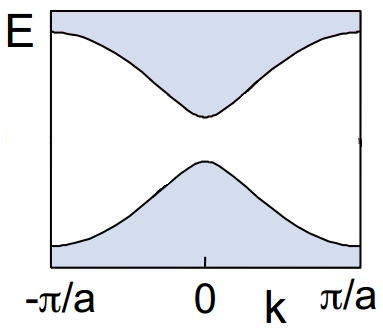
\includegraphics[width=0.5\linewidth]{diagrams/band_insulator_2.png}
				\caption{Free fermion band insulator}
			\end{figure}
			\begin{figure}
			\vskip-0.6cm
				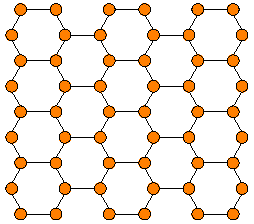
\includegraphics[width=0.5\linewidth]{diagrams/filled_honeycomb.pdf}
				\caption{Atomic picture}
				%Some integer number of localized orbitals filled, integer charge per site
			\end{figure}
		\end{block}
\end{column}
\begin{column}[T]{.5\textwidth}
	\begin{block}{Topological Insulators}
		\vskip-0.3cm
		\begin{figure}
			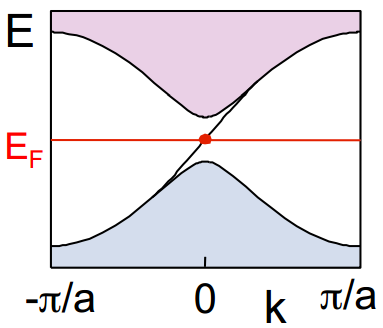
\includegraphics[width=0.5\linewidth]{diagrams/chiral_edge.png}
			\caption{Band insulator with chiral edge \footnotemark}
			%Not viewed as some integer number of orbitals filled per unit cell
		\end{figure}
		\begin{figure}
			\vskip-0.7cm
				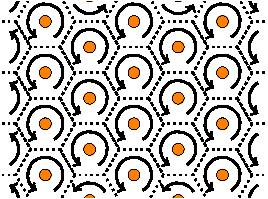
\includegraphics[width=0.5\linewidth]{diagrams/honeycomb_breakdown.pdf}
				\caption{Atomic picture breaks down}
		\end{figure}
	\end{block}

\end{column}
\end{columns}

\footnotetext[1]{
\citep{Hasan2010-fq}}

}
\end{frame}

%Examples include free fermion band insulators, both trivial and topological
%Interacting 1D examples would include the spin-1 heisenberg AFM
\begin{frame}{Construction of 1D Featureless Insulators}
\vskip-1.5cm		
\begin{columns}[T]
	\begin{column}[T]{.5\textwidth}
		\begin{block}{Classical Insulators}
			\vskip0.55cm
			\only<1, 2>{
			\begin{figure}
				
\includegraphics[width=\linewidth] {diagrams/trivial_chain.pdf}
				\caption{1D Trivial Chain}
			\end{figure}
			}
		 \only<3>{
			\begin{figure}
			  \vskip-0.5cm
				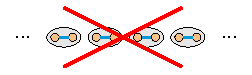
\includegraphics[width=\linewidth] {diagrams/trivial_chain_w_x.pdf}
				\vskip-0.4cm
				\caption{1D Trivial Chain}
			\end{figure}
			}
		\only<2>{
		\bi
		\item[] Product state with one boson per site
		\ei
		}
		\end{block}
	\end{column}
	\begin{column}[T]{.5\textwidth}
		\begin{block}{Topological Insulators}
			\vskip0.45cm
			\begin{figure}
				
\includegraphics[width=\linewidth] {diagrams/haldane_insulator_chain.pdf}
				\caption{1D Topological Chain}
			\end{figure}
		\only<2>{
		\bi
		\item[] Haldane Insulator Phase \cite{pollmann2010}
		\item Unitarily related to AKLT
		\item No $SU(2)$ symmetry
		\item Symmetry protected 2-fold edge degeneracy
		\ei
		}
		\end{block}
	\end{column}
\end{columns}
\only<1>{
\begin{center}
	\begin{figure}[]
		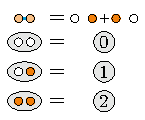
\includegraphics[width=0.4\textheight] {diagrams/haldane_insulator_chain_rules.pdf}
		\caption{Entangled pairs and projectors used in state construction}
	\end{figure}
\end{center}
}
\only<3>{
\begin{center}
	\begin{figure}[]
		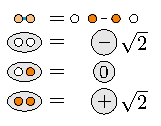
\includegraphics[width=0.4\textheight] {diagrams/aklt_rules.pdf}
		\caption{Entangled pairs and projectors for $SU(2)$ symmetric state}
	\end{figure}
\end{center}
}
\end{frame}

%Examples include free fermion band insulators, both trivial and topological
%Interacting 1D examples would include the spin-1 heisenberg AFM
\include{slides/theproblem}
\section{Entanglement Edge of Honeycomb Insulators}
\begin{frame}{Entanglement Spectrum}
\vskip-1.5cm
\only<1>{	
	\begin{figure}[hbctp]
	\begin{center}
	\includegraphics[width=\textwidth]{{EntanglementSpectrum_L10.pdf}}
	%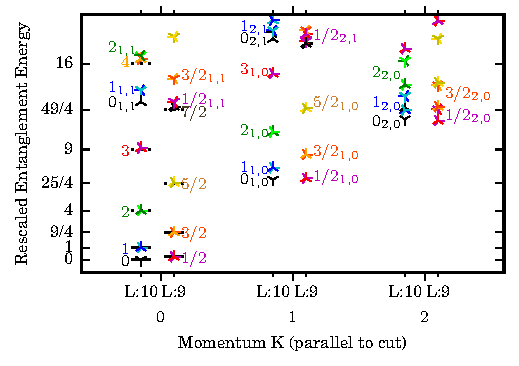
\includegraphics{{interpolatedboson/a10/plots/EEIdentify.pdf}}
	\end{center}
	\end{figure}
}
\only<2>{
	\begin{figure}[hbctp]
	\begin{center}
	\includegraphics[width=\textwidth]{{EntanglementSpectrum_L9.pdf}}
	%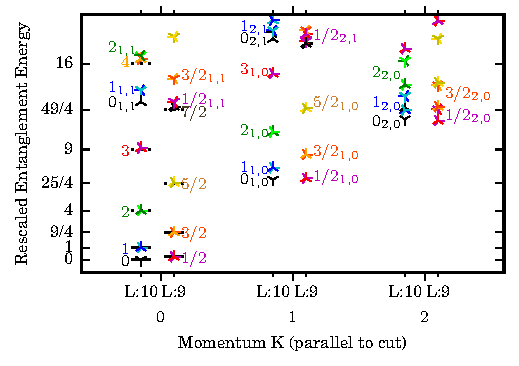
\includegraphics{{interpolatedboson/a10/plots/EEIdentify.pdf}}
	\end{center}
	\end{figure}
}
\end{frame}
\begin{frame}{Finite Size Analysis of Entanglement Spectra}
\vskip-1.5cm
%\begin{columns}[T]
%\begin{column}{.5\textwidth}
\only<1>{
        \begin{figure}[hbctp]
        \centering
        \includegraphics[width=0.8\textwidth]{{EntanglementEnergyScaling.pdf}}
        %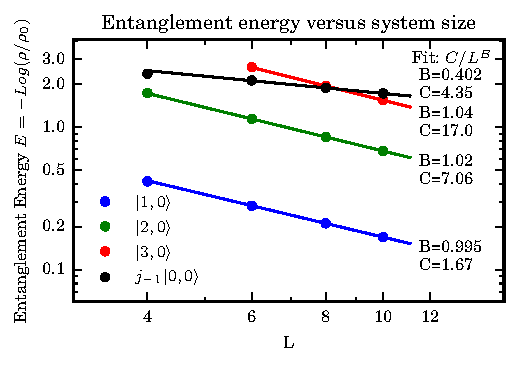
\includegraphics{{interpolatedboson/a10/plots/EntanglementEnergyScaling2.pdf}}
        %\caption{Power law fits for the lowest three states above the ground state at momentum zero and lowest two states at momentum 1 in Figure \ref{fig:sc-EEFinitesize}. The $1/L$ scaling is a signature of a gapless (entanglement) Hamiltonian. The labeling of the states $\ket{e, m}$ or $j_{-1} \ket{e, m}$ is explained in the CFT section below.}
        %\label{fig:sc-EEScaling}
        \end{figure}
%        \bi 
%        \item<1-> Low energy modes show gapless $1/L$ behavior
%        \ei
}
%\end{column}
%\begin{column}{.5\textwidth}
\only<2>{
				\begin{figure}[hbctp]
        \centering
        \includegraphics[width=\textwidth]{{TopologicalEntanglementEntropy.pdf}}
        \end{figure}
}
%\end{column}
%\end{columns}

\end{frame}
\begin{frame}{Identification of Edge CFT}
\vskip-1.5cm
\newcommand{\uL}{\mathbf{L_0}}
\newcommand{\bL}{\mathbf{\bar{L}_0}}

\only<1>{
\begin{block}{Conformal Charge via 'Nested Entanglement Entropy'}
\vskip-0.5cm
	\begin{figure}[hbctp]
	\centering
	\includegraphics[width=0.8\textwidth]{{EdgeGS_EntanglementEntropy.pdf}}
	%\caption{Entanglement entropy within the entanglement ground state of the soft-core boson state on $10$ sites. For comparison, the Cardy-Calabrese formula $S(x) = c/3 \log \sin( \pi x/L) + const.$ is shown with $c=\frac{1}{2}, 1,$ and $2$, with the $const.$ fixed by matching the maximum of the entanglement entropy data. $c=1$ is a good fit.}
	%\label{fig:hc-edge-gs-ee}
	\end{figure}
	\begin{empheq}[box={\mybluebox[4pt][4pt]}]{equation*}
	c = 1
	\end{empheq}
\end{block}
}

\only<2>{
\begin{columns}[T]
\begin{column}{0.35\textwidth}

\begin{block}{Conformal Weights}
We can match the rescaled entanglement energies to the conformal weights of a free bosonic CFT.

%\begin{tabular*}{\columnwidth}{@{\extracolsep{\stretch{1}}}*{2}{c}@{}}
%\begin{tabularx}{\columnwidth}{|X|X|}
%\toprule
%\small
%\begin{align*}
%	\mathbf{P} &=&\frac{2\pi}{L}(\uL-\bL) 
%	&=& \frac{2\pi}{L}(em + n - \bar{n}) \\
%	%\widetilde{\mathbf{P}}&= em + n - \bar{n} &\\ 
%	\mathbf{H} &=& \frac{2\pi}{L}(\uL+\bL) 
%	&=& \frac{2\pi}{L}(\frac{\kappa e^2}{2} + \frac{m^2}{2 \kappa} + \frac{n + %\bar{n}}{2}) %\\
%\end{align*}
%\normalsize

%\begin{empheq}[box={\mybluebox[4pt][4pt]}]{equation*}
%\mathbf{H} \propto e^2 + \frac{m^2}{\kappa^2} + \frac{1}{\kappa}(n + \bar{n})
%\end{empheq}
$$
\mathbf{H} \propto e^2 + \frac{m^2}{\kappa^2} + \frac{1}{\kappa}(n + \bar{n})
$$
\end{block}
%}

%\only<3>{
\end{column}
\begin{column}{0.65\textwidth}
\begin{block}{Conformal primary identification in entanglement spectra}
\begin{figure}[hbctp]
\begin{center}
\includegraphics[width=\textwidth]{{EEIdentify.pdf}}
%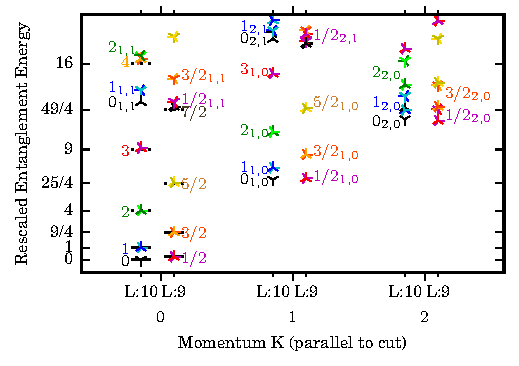
\includegraphics{{interpolatedboson/a10/plots/EEIdentify.pdf}}
\end{center}
%\caption{The identification of the states $\ket{e, m}_{n, \bar{n}}$ in the spectrum of the soft-core boson entanglement Hamiltonian. The label $e$ gives the U(1) charge. The labels $n$, $\bar{n}$ label the levels in the right or left-moving sectors of the Kac-Moody algebra. When the level $n$ is larger than 1, the level shows $Z(n)$ approximately degenerate states. The best estimate for the Luttinger parameter $\kappa = 1/6.4$ is given by the inverse of the energy of the $\ket{1, 0}_{1, 0}$ state. The label $m$ is 0 for all states shown - however, the primary states $\ket{e, m=\pm 1}$ can be seen centered around momentum $\pi$, with energies on the order of $1/(4\kappa^2)$.}
%\label{fig:primaries}
\end{figure}

\end{block}
\end{column}
\end{columns}
}

\end{frame}

\begin{frame}{Future Work}
\vskip-2cm

\begin{columns}[T]
    \begin{column}[T]{.9\textwidth}

\begin{block}{}
	\bi
	\item[] Entanglement properties with different geometries
		%Which entanglement cuts have exact spectrum degeneracy 
		%Which cuts give you a gapless mode in thermodynamic limit
		\bi
		\item Armchair cylinder edge %Preliminary results suggest
		\item Finite size clusters 
		\item Explain results for arbitrary geometries with tensor network properties, e.g. 'MPO injectivity'
		\ei
	\item[] Find a 2D local Hamiltonian and confirm with numerics
	
		\item[] \vskip-0.5cm $$H_{EBH} = \left(\sum\limits_{\varhexagon} \sum\limits_{i,j \in \varhexagon} -t b^{\dagger}_i b_j + V n_i n_j \right) +\mu N ?$$ 
	\item[] Physical properties of the phase
	\item[] Can we construct% or find obstruction to
	 an SU(2) symmetric FI?
	\ei	
\end{block}

    \end{column}
    \begin{column}[T]{.1\textwidth}
    \end{column}
\end{columns}
\end{frame}
\section*{}
\frame{
  \vspace{2cm}
  {\huge Questions?}

  \vspace{3cm}
  \begin{flushright}
    Brayden Ware

    \structure{\footnotesize{brayden@physics.ucsb.edu}}
  \end{flushright}
}

\frame{
  \vfill
  \centering
  \highlighton{
  \usebeamerfont*{frametitle}Bonus slides

  %\usebeamerfont*{framesubtitle}Bonus slides
  }
  \vfill
}

\begin{frame}
  \frametitle{Resources}
  \vskip-1.7cm
  %\framesubtitle{If you want to improve this style}
  \bibliography{references}
  %\beamertemplatearticlebibitems
\end{frame}


\end{document}
